\section{Evaluation design and denominators}
The experiments use three collections and four target quantities. SciFact supplies a reference for document relevance, claim verdict and sentence alignment \cite{SciFact}. NFCorpus supplies graded relevance judgments in the BEIR format \cite{BEIR}. The synthetic collection supplies designed relationships, time intervals and, for selected cases, a truth value known to the generator. There is no independent real-world source-dependency label in the scientific retrieval experiment.

\begin{center}\small
\begin{tabularx}{\linewidth}{@{}p{.30\linewidth}rX@{}}\toprule
Evaluation unit & Count & Target\\\midrule
SciFact abstracts & 5,183 & Fixed collection for retrieval and verification.\\
SciFact development claims with rationales & 188 & Rank of relevant abstracts, using a cutoff of ten.\\
All SciFact development claims & 300 & Four-way evidence verdict, including insufficient.\\
Initial neural diagnostic & 48 & Decisive decisions and citation alignment, seed 17.\\
Subsequent neural comparison & 80 & Same queries, three-document budget, filter on or off, seed 41.\\
NFCorpus test queries & 323 & Graded retrieval on 3,633 documents.\\
Synthetic test worlds & 360 & Verdict accuracy, dependency grouping and calibration after separate development and calibration partitions.\\\bottomrule
\end{tabularx}
\end{center}
The 48 and 80 neural sets do not overlap. Both are subsets of public SciFact development data. The original 300-claim evaluation had already contributed aggregate retrieval and rule-verifier measurements. The 48-claim diagnostic exposed poor citation alignment and motivated the passage filter. The 80-claim comparison therefore estimates behavior on a different set of neural queries within the same public collection. The private SciFact test set was never scored.

\subsection{Metrics and experimental controls}
For query $i$, let $R_i$ be its annotated relevant documents and $L_i^k$ the top-$k$ list. Recall is $|R_i\cap L_i^k|/|R_i|$. Precision divides the same numerator by $k$. Reciprocal rank is the inverse rank of the first relevant hit, or zero when no hit appears in the prefix. For relevance grades $g_{ij}$, nDCG discounts high-ranked gains by $\log_2(j+1)$ and divides by the ideal ordering under the judgments. SciFact uses binary relevance. NFCorpus uses graded gains. The reported values are means across eligible queries.

For verification, \emph{coverage} is the fraction of all queries receiving support or refutation. Overall accuracy counts exact agreement on all verdicts, including correct abstentions labeled insufficient. \emph{Decisive accuracy} divides correct decisive answers by all decisive answers. \emph{Citation alignment} counts emitted citations found within an annotated sentence of the appropriate document and stance. The last metric is micro-averaged over passages. A query with three citations has three opportunities to affect it. We also count queries with a correct verdict and at least one aligned citation to keep the unit of observation explicit.

Two baselines help interpret the denominators. A system that always predicts insufficient gets 112/300 SciFact development verdicts right and answers no claims. An extractive system that always returns the most similar sentence emits an answer to every query but can cite irrelevant evidence on queries with no annotated rationale. Reporting accuracy or citation count alone can make either behavior look useful for the wrong reason.

For the paired neural comparison the corpus, candidate encoder, reranker, page size, number of rounds, stance model and stance acceptance threshold are fixed. Only the optional rationale filter changes. For copy injection the full-evidence and truncated-evidence experiments deliberately use different review budgets. We avoid attributing differences between the 48-query and 80-query sets to a model change, because the composition of those sets differs.

\section{What retrieval recovers}
\begin{center}\small
\begin{tabular}{@{}lrrrr@{}}\toprule
SciFact method & Recall@10 & P@10 & MRR@10 & nDCG@10\\\midrule
BM25 & .930 & .100 & .785 & .816\\
Character LSA & .478 & .052 & .264 & .313\\
Rank fusion & .864 & .092 & .572 & .640\\
Fusion + learned relevance & .863 & .091 & .619 & .673\\\bottomrule
\end{tabular}
\end{center}
BM25 leads every column in this comparison. Mean Recall@10 of .930 describes the average fraction of annotated relevant abstracts recovered per eligible query. Precision@10 of .100 is compatible with retrieving approximately one relevant document per ten returned. An annotated-abstract task with few relevant documents per query has a low maximum attainable precision at a fixed cutoff. The high recall alone says little about the quality of the nine other passages a downstream verifier might inspect.

Relative to unweighted fusion, adding the learned head raises nDCG by about .033 and MRR by .047, while Recall@10 changes by about $-.001$. One plausible explanation is that it moves an already retrieved relevant document closer to the top. These aggregates cannot establish which individual rank changes account for the difference. Query-level paired ranks would be needed to identify that contribution exactly.

\begin{figure}[htbp]\centering
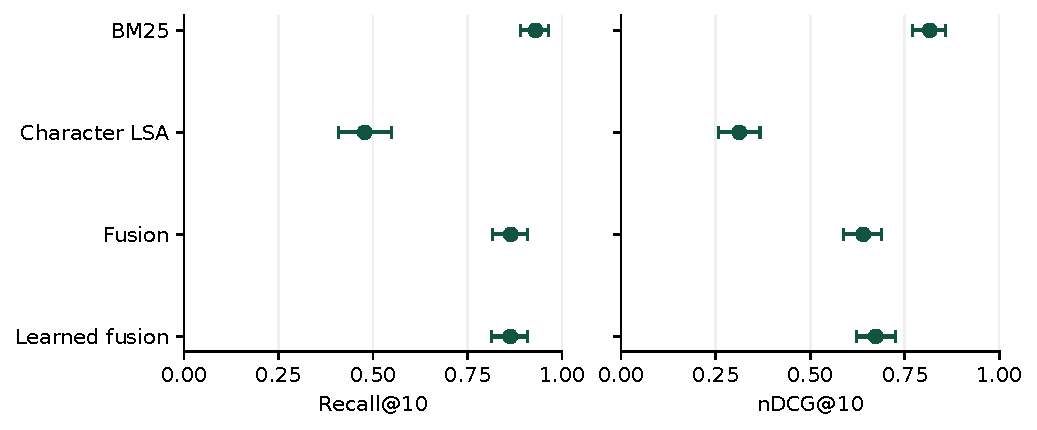
\includegraphics[width=\linewidth]{retrieval-intervals.pdf}
\caption{SciFact document retrieval over 188 queries. The bars are percentile intervals from 1,500 query bootstrap resamples in the published evaluation. Each interval concerns one method's mean. A test of a difference between methods would require the paired query-level differences.}
\end{figure}

The BEIR-format NFCorpus run provides a second retrieval task. With the default hybrid configuration, mean Recall@10 was .134, Precision@10 .198, MRR@10 .464 and nDCG@10 .264 on 323 test queries. Multiple relevant documents and graded judgments change both the difficulty and the attainable values. Precision can exceed the SciFact value while recall is much lower. Comparing these datasets as though the change measured a loss of verifier accuracy would mix two different targets. The NFCorpus run ends at ranked documents.

On the 48-query neural diagnostic, the 33 queries with annotated evidence had mean Recall@10 of .855. On the 80-query comparison, the 49 eligible queries had .980. Both are small subsets. Neural verification inspected only three documents per query, while the retrieval statistic examines ten. A correct hit at rank ten can contribute to the retrieval result even though it never enters the verification step. The change in sample composition and cutoff precludes treating either number as a direct explanation of answer accuracy.

\section{Controlled experiments on copying and time}
\subsection{How the synthetic worlds are constructed}
The generator produces 1,440 deterministic local worlds across twelve families. Each record supplies one query, a tiny document set, source-family labels, an optional evaluation date, an expected evidence verdict and a simulator truth value when defined. Development, calibration and test use 720, 360 and 360 distinct record IDs. Each test family contains 30 cases. Names and counts vary across worlds while the templates recur across partitions. A world is indexed separately so one station's observations cannot answer another station's query.

\begin{center}\small
\begin{tabularx}{\linewidth}{@{}lXr@{}}\toprule
Family & Perturbation or evidence target & Correct / 30\\\midrule
Copied error & Repeated opposition to one original observation. & 30\\
Independent reports & Two reports state the same count in distinct surrounding text. & 30\\
Syndication & A digest explicitly cites the earlier record. & 30\\
Conflict & Two eligible reports give incompatible numbers. & 30\\
Expired record & A later validity interval changes the answer at the requested date. & 30\\
False premise & A why-question presupposes an unestablished closure. & 30\\
Insufficient & A route map fails to give a berth count. & 30\\
Numeric disagreement & One eligible report supplies a different exact count. & 30\\
Multilingual & Spanish passage, English claim. & 0\\
Two-hop & Management identity and property occur in separate documents. & 0\\
Unsupported report & The available sentence supports a claim false in the simulator. & 30\\
Embedded instruction & An imperative attempts to supply an answer. & 30\\\bottomrule
\end{tabularx}
\end{center}
The last column measures agreement with the expected \emph{evidence verdict}. A score of 30 in the unsupported-report family means the system recognized what the visible report said. All thirty assertions were false in the generator's world. This is precisely the case in which substituting evidence accuracy for factual accuracy would reverse the interpretation.

Pairs drawn from the generated documents produced 330 true same-family decisions and 270 true different-family decisions, with zero observed false pair decisions. These are 600 document pairs induced by repeated templates, including multiple pairs per copied group. Their labels follow from the generator. They provide a unit-level check on grouping logic for the designed patterns. They do not validate authorship inference, independence of editorial desks, or the threshold for paraphrase detection in real reporting.

\subsection{Full visibility and multiplicity}
One observation supports a claim, a second opposes it, and each has strength one. Replicate the opposing report $n$ times, always leaving both observations visible. With grouping $S=C=1$ and $m=0$. In the ablated version each document has its own vote, so $S=1$, $C=n$ and
\[
             m_{\mathrm{naive}}=(1-n)/(2+n).
\]
At two copies the ratio of weaker to stronger weight is $1/2$ and the outcome remains conflict. At four copies it is $1/4$, below the .34 cutoff, and the system returns a refutation. A change in the unit of counting has changed the verdict even though no additional observation entered the collection.

\begin{figure}[htbp]\centering
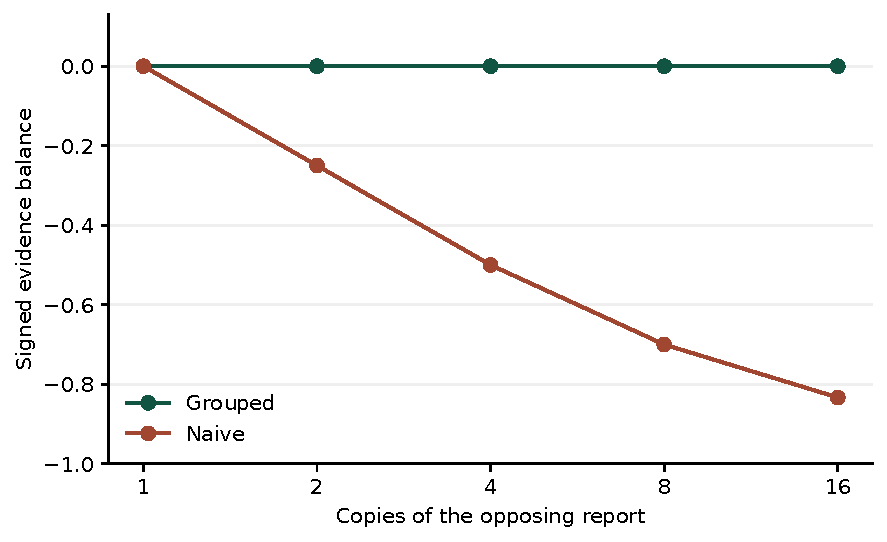
\includegraphics[width=.83\linewidth]{duplicate-injection.pdf}
\caption{One supporting observation and one opposing observation repeated across documents. All sources are available to the verifier. The grouped curve stays at zero. Naive voting reaches $-15/18$ with sixteen copies.}
\end{figure}

This intervention holds stance interpretation unusually stable. The repeated text is identical. The test gives the grouping method ample opportunity to identify it. A more difficult intervention would preserve the underlying report but change the text, citation links and publication metadata independently. That would test whether the grouping rule can still recognize the dependency. It is a separate question from the algebraic behavior once the component assignment is correct.

\subsection{Candidate crowding}
A second experiment places the query text in the title of each opposing copy, with a narrower title on the primary observation. The hybrid retriever ranks the competing documents, then verification examines at most two new records per round. The candidate set can change as copies are added. The table gives the verdict and number of documents examined. It reports actual runs and therefore includes early exhaustion when fewer records exist than the budget permits.

\begin{center}\small
\begin{tabular}{@{}rlll@{}}\toprule
Opposing copies & 1 round & 2 rounds & 5 rounds\\\midrule
1 & conflict (2) & conflict (2) & conflict (2)\\
2 & refuted (2) & conflict (3) & conflict (3)\\
4 & refuted (2) & refuted (4) & conflict (5)\\
8 & refuted (2) & refuted (4) & conflict (9)\\
16 & refuted (2) & refuted (4) & refuted (10)\\\bottomrule
\end{tabular}
\end{center}
With eight copies and five rounds, the ninth inspected document restores the competing observation. With sixteen copies and the same budget, ten examined documents can all descend from one side. This creates the same visible evidence as a collection containing just that side. No downstream operation over the visible records can reconstruct the missing primary report. A policy that diversifies candidate families before the cutoff addresses a different intervention from one that caps votes after the cutoff.

The experiment demonstrates an existence counterexample. It does not estimate the frequency of this failure in search traffic. The titles and copy counts deliberately favor displacement. A prevalence study would need an independently sampled population of stories, time-stamped documents, a realistic distribution of duplicate counts and a documented search budget. The controlled experiment is valuable because it specifies what such a study should count: the rank of the first eligible observation from each independent family.

\subsection{Ablation and synthetic calibration}
\begin{center}\small
\begin{tabular}{@{}lrrr@{}}\toprule
Configuration & Correct / 360 & Decisive / 360 & Mean rounds\\\midrule
Full rule pipeline & 300 & 150 & 1.0\\
Document votes & 270 & 180 & 1.0\\
Time eligibility removed & 270 & 120 & 1.0\\
Contradictions ignored & 180 & 150 & 1.0\\
Fixed budget & 300 & 150 & 1.0\\
Final check removed & 300 & 150 & 1.0\\
BM25 verification & 300 & 150 & 1.0\\
LSA verification & 300 & 150 & 1.0\\\bottomrule
\end{tabular}
\end{center}
Removing grouping converts repeated opposition into additional decisive answers. Removing time eligibility permits stale evidence to compete and reduces coverage. Both variants lose thirty correct verdicts, with opposite changes in coverage. On these small worlds the adaptive stopping and final-offset ablations produce no accuracy gain. The null result matters: we cannot attribute a benefit to either mechanism from this table. Some unsupported inputs take zero rounds and some worlds need two, even though the mean is one.

Isotonic calibration uses only calibration-world answers for which a simulator truth value exists. The fitted map has two knots, $.5\mapsto .75$ and $2/3\mapsto 1$. On the 150 eligible decisive test responses, the Brier score is .150. Thresholding at .75 covers 150/360 queries with error rate .20 among answers. At 1.0 it covers 30/360 with zero observed errors. The ten-bin expected calibration error is zero on this template-balanced partition. Repeating the same template mixture in calibration and test makes such agreement possible. A change in the frequency of false unsupported reports alone could break it while leaving the software unchanged.

\section{Scientific verdicts and citation alignment}
\subsection{The initial diagnostic}
The rule pipeline abstained on all 300 scientific development claims. It received credit on the 112 gold insufficient cases. Literal rules are well matched to exact template statements but cannot cover many scientific paraphrases. The original neural diagnostic issued 24 decisive answers on 48 claims. Ten of the 24 matched the gold verdict. Among 39 citations, two aligned to an annotated rationale of the right stance. Thus half the sample received an answer while only two answered claims had an aligned citation.

The diagnostic motivated a narrower question than general NLI improvement: can a relevance filter suppress stance decisions about unrelated sentences? The next comparison adds that filter while retaining the same three-document retrieval budget. The low precision of the original diagnostic also motivates reporting counts of correct, cited claims. A filter can remove many poor citations and increase the alignment rate while retrieving no additional usable evidence.

\subsection{Paired replay on the 80-claim subset}
For this expanded edition we replayed both configurations on the 80 saved IDs and retained the per-query decisions and citation counts. All 80 gated records reproduced the archived triple of verdict, citation count and number of rationale matches. This replay adds paired information absent from the first report. The same claims were used again for analysis, so these data constitute a replication of the comparison and a deeper audit of its errors.

\begin{center}\small
\begin{tabular}{@{}lrr@{}}\toprule
Quantity on the same 80 claims & Ungated & Gated\\\midrule
All verdicts matching gold & 32 & 38\\
Decisive answers & 53 & 18\\
Correct decisive answers & 22 & 11\\
Incorrect decisive answers & 31 & 7\\
Correct decisive answers with an aligned citation & 6 & 6\\
Emitted citations & 83 & 19\\
Citations aligned to gold & 6 & 6\\\bottomrule
\end{tabular}
\end{center}
Coverage changes from 66.25\% to 22.5\%. Among decisive answers, agreement rises from 22/53 (41.5\%) to 11/18 (61.1\%). Citation alignment rises from 6/83 (7.2\%) to 6/19 (31.6\%). Each configuration delivers a correct verdict with at least one aligned citation on six of the 80 queries. The filter's clearest benefit in this sample is that the user receives fewer erroneous decisive answers and far fewer unmatched citations. The price is the loss of eleven correct decisive answers in aggregate.

\begin{figure}[htbp]\centering
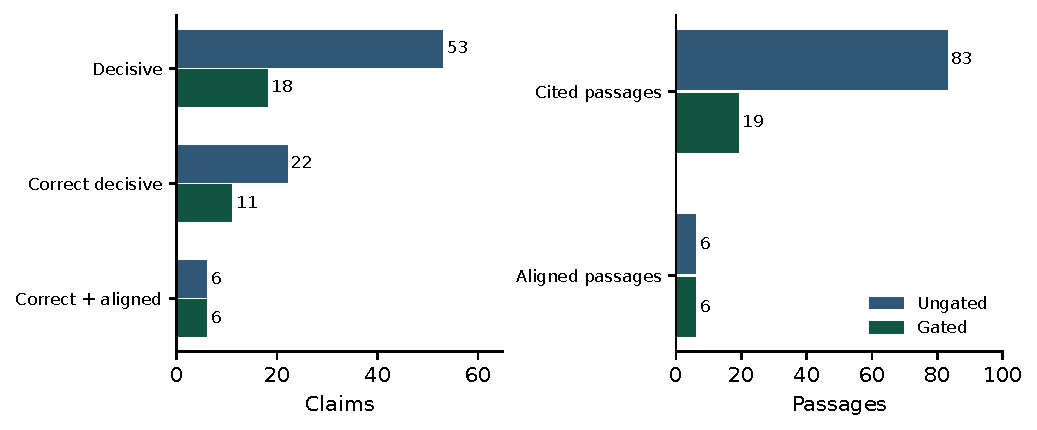
\includegraphics[width=\linewidth]{paired-grounding.pdf}
\caption{Decisive answers, correct answers and aligned passages in the paired replay. The numerator of citation alignment remains six as its denominator falls from 83 to 19. Left panel counts claims, right panel counts passages.}
\end{figure}

There are 20 claims where both verdicts agree with gold, 30 where both disagree, 18 where only the gated system is correct and 12 where only the ungated system is correct. Under the null of symmetric directions among the 30 discordant correctness pairs, the two-sided exact binomial test gives $p=.362$. The observed six-claim difference does not establish a population-level improvement. Claims may also share studies and topics. Treating the decisions as paired addresses reuse of a query across configurations, while further dependence across queries can still matter.

For the gated system the Wilson 95\% interval for 11/18 correct decisive answers is [.386,.797]. That broad interval describes sampling uncertainty under the usual binomial interpretation. It excludes neither substantial error nor materially better conditional accuracy. Treating the 19 citations as independent observations would additionally ignore clustering within answers. The tables provide direct counts so readers can choose an appropriate resampling unit for a larger replication.

\subsection{Direction of error}
\begin{center}\small
\begin{tabular}{@{}lrrr|r@{}}\toprule
Gold $\backslash$ gated prediction & Supported & Refuted & Insufficient & Total\\\midrule
Supported & 6 & 3 & 23 & 32\\
Refuted & 0 & 5 & 12 & 17\\
Insufficient & 1 & 3 & 27 & 31\\\midrule
Total & 7 & 11 & 62 & 80\\\bottomrule
\end{tabular}
\end{center}
The gated verifier labeled 62 queries insufficient. Twenty-seven were gold insufficient and 35 had an annotated decisive stance. Four of the 31 gold insufficient cases received a decisive answer. Three of 32 gold supported claims received the opposite polarity. A downstream editorial policy that reviews only refutations would encounter five correct refutations out of eleven issued. One that reviews supported answers would encounter six gold supports out of seven. These are very small denominators and should accompany any percentages.

The most common change under gating was refutation to insufficient (32 cases). Four supports became insufficient, and two conflicts changed, one to support and one to insufficient. The remaining 42 verdicts stayed the same. This pattern is compatible with a filter suppressing many refuting passages. It also shows that suppressing a passage need not reduce decisiveness: removing one side of a conflict can expose a surviving stance. A decision policy should inspect the passages removed on both sides before attributing a one-way improvement to stricter acceptance.

\subsection{Claim-level audit examples}
The following IDs refer to public SciFact development records and identify decisions that a reader can inspect. They illustrate different relationships between verdict and citation quality. The judgments concern benchmark annotations, not medical guidance. \cite{SciFact}

\begin{center}\small
\begin{tabularx}{\linewidth}{@{}rXX@{}}\toprule
ID & Gated result & Interpretation of the record\\\midrule
179 & Supported, one citation matched & Verdict and selected rationale both agree with the annotation.\\
539 & Supported, zero of one matched & Correct verdict, but the cited passage fails the gold alignment rule.\\
1144 & Refuted, zero of two matched & Several citations can accompany the correct label without identifying an annotated rationale.\\
1298 & Refuted, zero of one matched & The annotated verdict is supported. The filtered model retains the wrong polarity.\\
1292 & Refuted, zero of one matched & The reference marks evidence insufficient. Filtering reduces citation count from three to one while retaining the decisive error.\\\bottomrule
\end{tabularx}
\end{center}
Case 539 concerns a reported association between hypoglycemia and dementia risk. The verdict label alone would reward this output. An auditor who needs to trace the association back to the annotated scientific sentence receives weaker evidence. Case 1144 concerns a claim about beverage taxation. A source can be topically relevant to taxation yet fail to establish the particular incidence outcome in a claim. The saved result establishes a rationale mismatch. Determining whether the selected passage is an acceptable alternative requires reading the text, not simply counting it as factually false.

Case 1298 illustrates a more serious benchmark error. A claim containing negation receives a refutation where the gold label is support. The saved counts identify the error but do not establish whether it originated in sentence selection, truncation, or NLI. A causal diagnosis would need paired passages, model inputs and controlled substitutions. We deliberately distinguish what a prediction record establishes from an explanation that requires further inspection.

\subsection{Extractive comparators}
An additional baseline selects a sentence from four retrieved documents by token overlap. BM25 selects a gold rationale on 44/300 queries, the character-LSA retriever on 17/300, and hybrid fusion on 32/300. All three emit on every query, including the 112 with no gold rationale. The alignment test in this experiment checks the annotated sentence location. It does not condition the extraction count on a predicted stance as the neural citation metric does.

A rule-based verification filter on the hybrid extractor emits zero answers. A separate-search proxy issues another local query for the selected sentence and seeks verbatim corroboration outside its source component. It also emits zero and uses 600 retrieval operations for the 300 inputs. This experiment tests a restrictive local search-and-check rule inspired by one aspect of SAFE \cite{SAFE}. It omits the official evaluator's language-model decomposition and web-search protocol. The null outcome shows the cost of requiring independent literal agreement in scientific prose.
